\documentclass[conference,9pt]{IEEEtran}
\usepackage{color}
\usepackage{cite}
\usepackage{epsfig}
\usepackage{amssymb}
\usepackage{amsmath}
\usepackage{graphicx}
\graphicspath{ {../} }

\begin{document}
%\tableofcontents
%\textheight=22.6cm
%
% paper title
\title{Practical 1}

% author names and affiliations
\author{
  \IEEEauthorblockN{Albert Acebron}
  \IEEEauthorblockA{NIU: 1458626}
}


% make the title area
\maketitle
\begin{abstract}
  In this practical we will implement a digital decoder, which will be used it to decode a signal that was encoded using an unknown constellation and has been distorted by AWGN noise and the doppler effect
\end{abstract}



%----------------------------------------------------------------
% SECTION #1 
\section{Introduction}
Here we are presented with a received signal that needs to be decoded, of which we know the frequency and form of the pulse that was originally used to encode the information, along with the rate at which the doppler effect distorted the signal.

With these nibbles of information we will tackle the task at hand by first removing all noise and distortion from the signal and then proceeding to separate the pulses into the original data.

\section{Distortion removal}
If we take a look at the process that the signal has gone through before we received it we would see something like this\footnote{Note that this image is not meant to be a perfect representation of reality (eg: doppler effect and AWGN noise would probably be applied at the same time, not sequentially) but it's purpose is to illustrate the general process the signal goes through}:

\vspace{5mm}
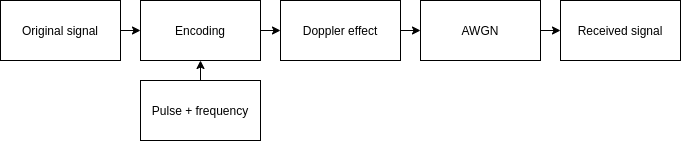
\includegraphics[scale=0.35]{initial-process.png}
\vspace{5mm}

So, logically, we will start by first removing the AWGN noise and, afterwards, tackle the distortion caused by the doppler effect.

\subsection{AWGN noise removal}
We know the pulse that was used for encoding was SQRCC, which has the following shape\footnote{Code used to generate this graph can be found on the Appendix}:

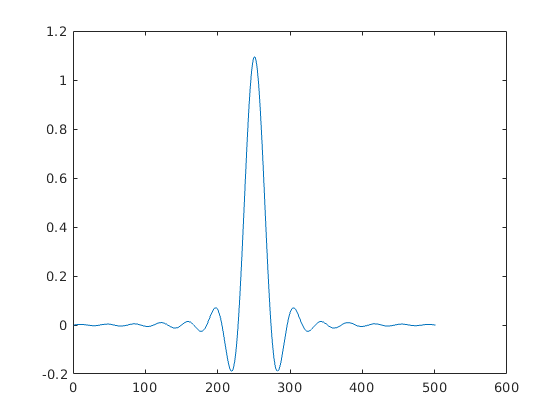
\includegraphics[scale=0.6]{pulso1}

And with this information we can construct a matched filter, which, when convoluted with the input signal, will generate an output signal that has a maximum SNR (under the assumption that AWGN is causing interferences)\cite{matched}.

This can be proved by taking the definition of convolution and SNR, formulating SNR as a function of the filter being applied, and then optimizing that. Doing so will yield that the filter that achieves this optimuum is a conjugated and time-reversed version\cite{proof} of the signal we are trying to match/find, which in this case is the SQRRC pulse.

In conclusion, the filter we should use is a conjugated and time-reversed SQRRC pulse, but this specific pulse doesn't have any imaginary components, so there's no need to conjugate it. For that reason we will simply revert it on the time scale, which should wield the same figure, since the pulse is symmetric against x=0.

Now that we have the shape of the filter, we'll modify it's scale to make it's total energy unitary, as that should normalize the average energy of the signal obtained after applying the filter\footnote{Numeric verification of this is on the Appendix}.

Since this transformation only involves scaling, we will apply it by introducing a linear multiplicative constant $\beta$:
$$newSignal = signal\cdot \beta$$

And, by the definition of signal energy\cite{energy}, the energy of the new signal will be:
$$energy = \sum (signal\cdot \beta)^2$$

Now we can constraint $energy$ to be 1 (what we want) and solve for $\beta$:
$$1 = \sum (signal\cdot \beta)^2$$
$$1 = \dfrac{\sum signal^2}{\dfrac{1}{\beta^2}}$$
$$\beta^2 = \dfrac{1}{\sum signal^2}$$
$$\beta = \sqrt{\dfrac{1}{\sum signal^2}}$$

Which evaluates to 0.2\footnote{The code used to calculate this value is on the Appendix}.

In conclusion, the amplitude of the filter will be multiplied by 0.2 to get it's total energy to be 1.

At this point we've obtained the filter and we could just apply it directly to our input signal by doing a convolution with it. However, convoluting a long signal is very expensive computationally, so instead we'll do that with the overlap-add algorithm\cite{overlap}, which is based on the idea of cutting up a long signal into chunks, performing the convolution with each of them separately and merging all the results together afterwards.

\pagebreak
The following is the implementation of the overlap-add algorithm that was used to apply the filter to the input signal\footnote{The code used to apply the filter along with a correctness test can be found on the Appendix}:
\begin{verbatim}
  function FilteredSignal = 
    overlap_add(RxSignal, h)

  M=length(h);
  Lr=length(RxSignal);
  % Taken from the recomendation
  % on the practical
  L=(M-1)*2;
  N=L+M-1;
  Hx=fft(h, N);
  FilteredSignal=zeros(Lr+M-1, 1);
  
  for x = 0:floor(Lr/L)
      len=L;
      initialPos=x*L+1
      if (initialPos+len)>(Lr-1)
          len=Lr-initialPos
          N=len+M-1;
          Hx=fft(h, N);
      end
      r=RxSignal(initialPos:initialPos+len-1);
      Rm=fft(r, N);
      Ym=Rm.*Hx;
      ym=ifft(Ym, N);
      endFiltered=initialPos+length(ym)-1;
      FilteredSignal(initialPos:endFiltered)=
        FilteredSignal(initialPos:endFiltered)
        +ym;
  end
\end{verbatim}
  
\subsection{Removal of Doppler effect}
Now that the AWGN noise has been minimized, we should be left with a signal that can be expressed as:
$$r[n]=s[n]\cdot e^{jwn}$$
Where $s[n]$ is the signal that was sent by the receiver and the one we wish to obtain, while the $e^{jwn}$ terms are distorsions caused by the doppler effect.

Luckily, given that the change caused by the doppler effect just translates into a set of multipliers that are applied to each output value, these can be cancelled by multiplying every value by it's corresponding multiplicative inverse, that is:
$$s[n]\cdot e^{jwn} \cdot e^{-jwn} = s[n]$$

The only thing that's left is to calculate the value of $w$, and we know that $F_d$, the doppler frequency, is equal to $50$, along with the fact that the time difference between each sample is $\dfrac{1}{F_s}=5*10^{-8}$, so the frequency shift experienced between samples will be $\dfrac{F_d}{F_s}$, which converted to angular frequency is $w=2\pi f=2\pi \dfrac{F_d}{F_s}$, meaning that each sample value will need to be multiplied by $e^{\dfrac{-jn2\pi F_d}{F_s}}$ where n is an increasing counter\footnote{Implementation in Appendix}.



\section{Detection}
At this point we've already removed noise and interferences from the signal, so now we'll tackle the second half of our DSP pipeline. More concretely, we will decode the signal down to the symbols that were originally sent.

\subsection{Decimation}
In it's current state, the signal we have contains $N_{ss}=F_s \cdot T_{sym}=20\cdot10^6 \cdot 10^{-6} = 20$ samples for every symbol sent, so it's clear to see that, as we only want to obtain the value of the symbol, we have a lot of extraneous information that we could get rid of.

Diving deeper, we can consider that, because the modulation used here is amplitude-based, we are mostly interested in the samples that have the highest value among the ones that pertain to the same symbol, as those will display the highest absolute difference between possible symbol values\footnote{The intuition behind this is that, in an scenario where one sample corresponding to a symbol has the value 0.05 while another corresponding to another symbol has 0.1, an error of 0.3 would lead to misclassification, whereas if the value of those samples were 5 and 10 the error would need to be 10 times bigger, thus misclassification is more unlikely to happen}, thus minimizing error when they are classified/decided.

Given that the signal we are handling has a period of $N_{ss}=20$, it's trivial to see that peaks will appear every 20 samples, thus that should be the period used for decimating, that is, between each value sampled there will be 19 that will be left out. The problem here is how to pick the offset from which to start sampling, as we have to take into account the changes applied in the previous steps, such as the convolution with a matched filter.

To do that let's remember that the matched filter is just a scaled version of the pulses that make up our input function, so if we plug that into the definition of convolution\cite{conv} (using a single pulse for now):
$$y(t)=\sum_{k} p(k)p(t-k)$$
We see that what we have here are multiplications of two values, which, due to the growth curve of x*y, will grow much faster the higher the values are. Following that intuition it should be easy to see that the sum will be highest when the two functions match exactly.

Now if we consider that our pulse is symmetric against axis $x=\dfrac{N}{2}$ when $0\leq k\leq N$ we can conclude that the functions will match ($k=t-k$) when $t=N$.

This may have been a bit hand-wavy, but if we look at a set of SQRRC pulses (blue) and it's convolution with another SQRRC pulse we can verify that it holds true:

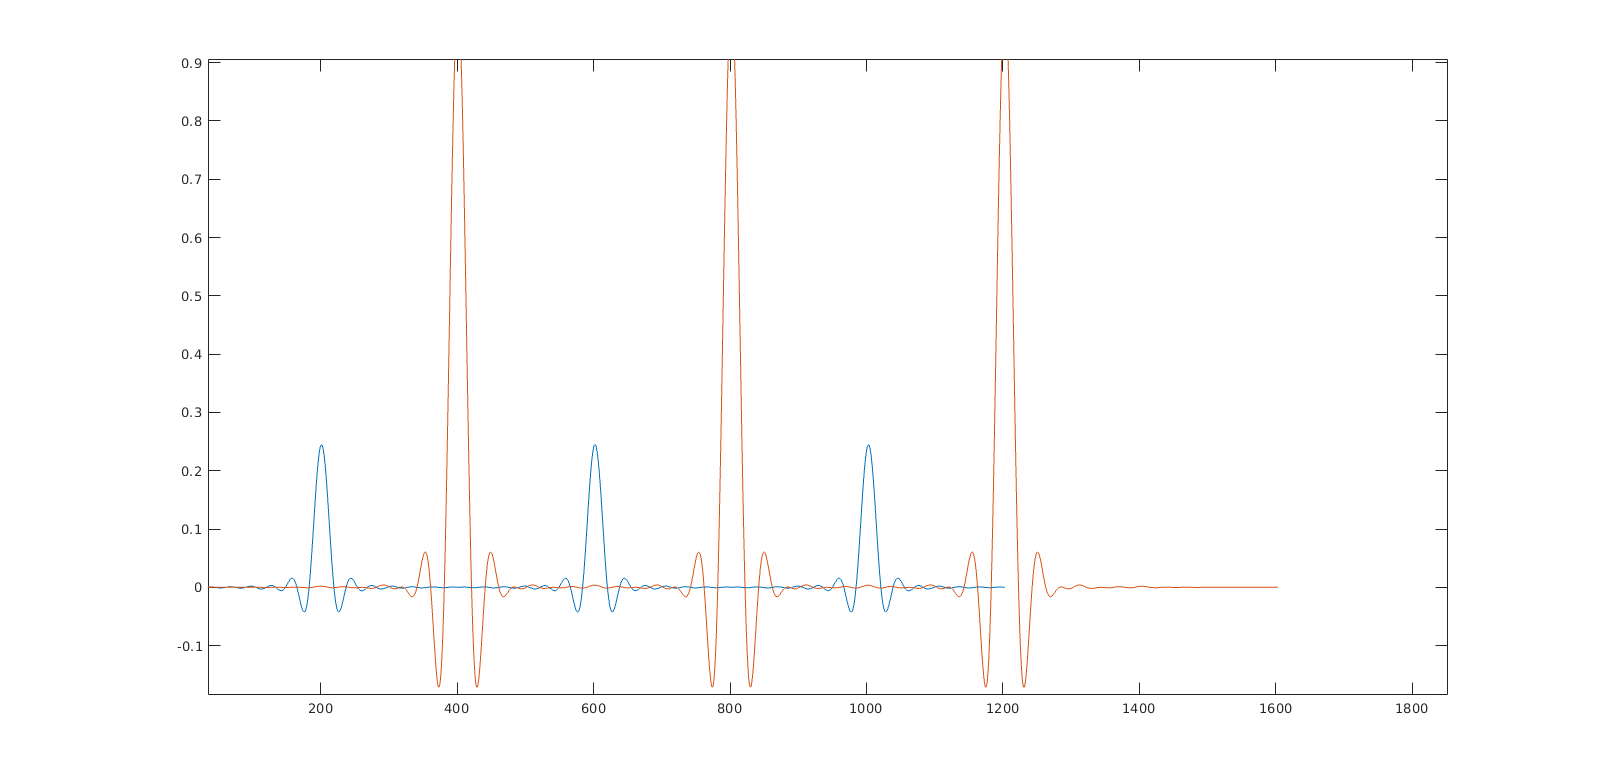
\includegraphics[scale=0.23]{convs}

In conclusion, we will decimate our signal at each 20th sample\footnote{See Appendix for code}.


\subsection{Detection}
If we now graph the resulting signal we'll end up with:

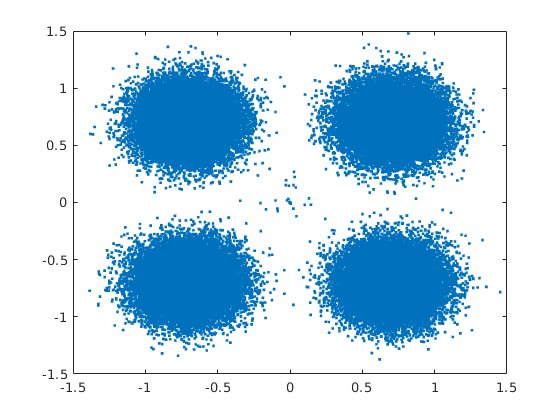
\includegraphics[scale=0.6]{res}

Looking at it we can clearly see that the constellation is a quaternary construction, where four symbols have been encoded into four different quadrants. The values at the center of the graph generally correspond to the ones at the start or end of the signal, as it's tails (aprox 100 samples) have low amplitude.

Now that the constellation that we are dealing with is known\footnote{Including the fact that the 4 ideal points are located at $(\pm\sqrt{\dfrac{1}{2}}, \pm\sqrt{\dfrac{1}{2}})$}, we can classify each of the samples into one of the four possible values to get back the message that was sent. We will do this by assigning each sample to the ideal value that it's more likely to be representing thus minimizing errors. In practical terms this means that we'll be splitting the sample using the x and y axis\footnote{It can be proved that this split generates a classification that minimizes the chances of symbol misclassification. We won't provide the whole proof here but the intuition is that error is minimized when a sample is classfied as the ideal point that is closest to it, and for any point in one of the quadrants the closest of the ideal points will be the one on the same quadrant}.

The following code applies this classification method:
\begin{verbatim}
function DetSymbols = symDetector(
  DecimatedSignal)

angles=atan2(imag(DecimatedSignal),
 real(DecimatedSignal));
DetSymbols=zeros(length(angles),1);
l=sqrt(1/2)

for i=1:length(angles)
    a=angles(i);
    if a>0
        if a<(pi/2)
            DetSymbols(i)=l+ l*j;
        else
            DetSymbols(i)=-l+ l*j;
        end
    else
        if a<(-pi/2)
            DetSymbols(i)=-l -l*j;
        else
            DetSymbols(i)=l -l*j;
        end
    end
end
\end{verbatim}

This results in the following graph when the samples are colored by classification\footnote{See Appendix for code}:

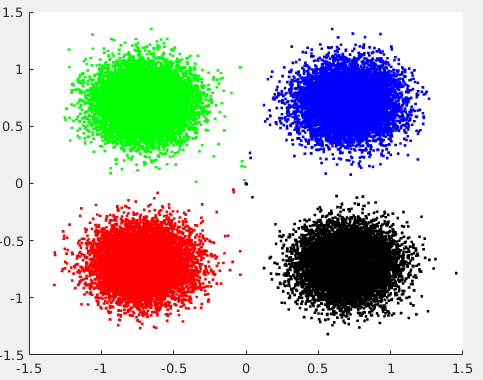
\includegraphics[scale=0.5]{class}

\section{Conclusion}
We managed to remove noise through a matched filter, cancel the distortion caused by the doppler effect and decode the signal while minimizing errors through the whole process, thus accomplishing the task of building signal processing pipeline that can decode the received signal.

\section{Appendix}
Note: All the code snippets provided in this document have had their lines wrapped to prevent visual overflows.
\subsection{Code used to generate the graph of the SQRRC pulse}
\begin{verbatim}
senyal_conformat = pam_sqrrc(25, 20, 0.35, 1)
plot(1:length(senyal_conformat),
    senyal_conformat)
\end{verbatim}

\subsection{Calculation of $\beta$}
\begin{verbatim}
  beta = sqrt(1/sum(senyal_conformat.^2))
\end{verbatim}

\subsection{Application of overlap-add}
\begin{verbatim}
  filter = pam_sqrrc(20, 20, 0.35, 1);
  energy = sum(filter.^2)
  filter = filter/sqrt(energy);
  output = overlap_add(RxSignal, filter)
\end{verbatim}

\subsection{Verification that the overlap-add implementation is correct}
Given that the overlap-add method we implemented before is just an alternate way of performing a convolution, we will check it's correctness by comparing it's output with the output of a normal convolution. To do that we'll generate two triangular pulses, convolute them with different methods and graph the outputs together:
\begin{verbatim}
t1=triang(10)
t2=triang(30)
hold on
plot(conv(t2,t1))
plot(add(t2,t1))
\end{verbatim}

The resulting plot is the following, it is not clear but the two superimposed figures are right on top of each other, meaning that the two methods are equivalent\footnote{This afirmation has only been proved for the specific case under test} and our implementation of overlap-add is correct when used on these signals.

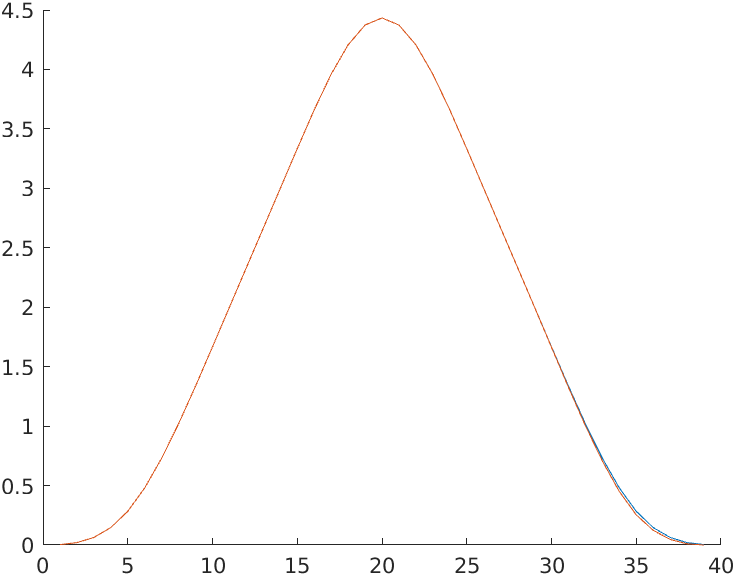
\includegraphics[scale=0.6]{comp}

\subsection{Verification of the output signal's average energy}
This is achieved by applying the energy calculation performed in the previous practical to the absolute values ($\sqrt{real^2+imag^2}$) of the complex numbers obtained from the convolution.

\begin{verbatim}
output = add(RxSignal, filter)
avg_energy = sum(imag(output).^2 
+ real(output).^2)/length(output)
\end{verbatim}

Which results in an average energy of 0.96. We've also checked the output comparing it with the result of "conv(RxSignal, output)" and the length is the same.

\subsection{Removal of doppler effect}
\begin{verbatim}
  n=1:length(output)
  no_doppler = output.*exp(-i*100*pi*n'*50e-9)
\end{verbatim}

\subsection{Code for decimation}
\begin{verbatim}
  DecimatedSignal=no_doppler(20:20:end)
\end{verbatim}

\subsection{Code for graphing the post-decimation signal}
\begin{verbatim}
  plot(DecimatedSignal + 1i * eps, ‘.’);
  axis square;
\end{verbatim}

\subsection{Average energy of the constellation}
Given that we are dealing with a quaternary constellation, we know that ideally all points should be the same distance away from the center, so their energy will be also the same. Now, the average energy needs to be 1 and all samples should have the same energy so it's easy to see that the energy for each of them will need to be 1.

For that to happen, the imaginary ($img$) and real ($rea$) parts of symbol must meet the following identity:
$$img^2+rea^2=1$$

And due to how the points are ideally distributed, this can only happen  if:
$$abs(img)=abs(rea)=\sqrt{\dfrac{1}{2}}$$

So the symbols will all need to be of the form $(\pm\sqrt{\dfrac{1}{2}}, \pm\sqrt{\dfrac{1}{2}})$.

We can find the average energy of the constellation with:
\begin{verbatim}
avg_cons_energy=sum(imag(DecimatedSignal).^2
  + real(DecimatedSignal).^2)/length(DecimatedSignal)
\end{verbatim}

Which resolves to 1.047, thus the average energy of the constellation is not strictly unitary but it is quite close to that.

\subsection{Code for coloring based on classification}
This is a fork of the symDetector function provided before:
\begin{verbatim}
angles=atan2(imag(DecimatedSignal),
  real(DecimatedSignal));

hold on;
color=""
for i=1:length(angles)
    a=angles(i);
    if a>0
        if a<(pi/2)
            color="b.";
        else
            color="g.";
        end
    else
        if a<(-pi/2)
            color="r.";
        else
            color="k.";
        end
    end
    plot(DecimatedSignal(i) + 1i * eps, color);
end
\end{verbatim}


\begin{thebibliography}{1}

  \bibitem{matched}
  https://www.mathworks.com/help/phased/ug/matched-filtering.html,
  retrieved on 7/10/20

  \bibitem{proof}
  https://en.wikipedia.org/wiki/Matched\_filter\#Derivation\_via\_matrix\_algebra,
  retrieved on 6/10/20

  \bibitem{energy}
  https://en.wikipedia.org/wiki/Energy\_(signal\_processing),
  retrieved on 7/10/20

  \bibitem{overlap}
  https://en.wikipedia.org/wiki/Overlap\%E2\%80\%93add\_method,
  retrieved on 7/10/20

  \bibitem{conv}
  https://en.wikipedia.org/wiki/Convolution\#Discrete\_convolution, 
  retrieved on 9/10/20
\end{thebibliography}

% that's all folks
\end{document}


